\documentclass[a4paper, 12pt]{article}
\usepackage[utf8]{inputenc}
\usepackage{newpxtext, newpxmath}
\usepackage[breaklinks=true]{hyperref}
\usepackage{graphicx}
\usepackage{caption}
\usepackage[left=3cm, right=2cm, top=3cm, bottom=2cm]{geometry}
\geometry{a4paper}
\usepackage{fancyhdr}
\usepackage[brazilian]{babel}
\usepackage{siunitx}
\usepackage{float}
\pagestyle{fancy}
\renewcommand{\headrulewidth}{0pt} 
\lhead{}\chead{}\rhead{}
\lfoot{}\cfoot{\thepage}\rfoot{}
\graphicspath{{../figures/}}
\sisetup{output-decimal-marker={.}}
\usepackage{amsfonts}
\usepackage{mathtools}
\usepackage{cleveref}
\usepackage{spverbatim}
\usepackage{setspace}
\setlength{\parskip}{1em}
\singlespacing

\newcommand{\empt}[2]{$#1^{\langle #2 \rangle}$}

\usepackage{amsmath}

\usepackage{tikz}
\usetikzlibrary{shapes,arrows,fit, positioning, arrows.meta}
\usetikzlibrary{backgrounds}
\usepgflibrary{shapes.multipart}
\def\layersep{2.5cm}
\def\layersepp{5cm}	

\begin{document}
\begin{titlepage}
\newcommand{\HRule}{\rule{\linewidth}{1.5mm}}
	
\center


\includegraphics[width=0.15\textwidth]{logo-unicamp.pdf}\\[1.0cm]

\textsc{\Large Estágio Científico e Tecnológico I - EE015}\\[0.5cm]

\textsc{\large Relatório}\\[1.5cm]

{\Large \bfseries Predição de Séries Temporais Baseada em Redes Neurais Artificiais}\\[2.5cm]

\begin{flushleft}
Submetido à \\ Faculdade de Engenharia Elétrica e Computação (FEEC)\\[1.5cm]

Departamento de Engenharia de Computação e Automação Industrial (DCA)\\
Faculdade de Engenharia Elétrica e de Computação (FEEC)\\
Universidade Estadual de Campinas (UNICAMP)\\
CEP 13083-852, Campinas - SP\\[1.0cm]

Aluno: João Pedro de Oliveira Pagnan\\
Orientador: Prof. Levy Boccato \\[4.5cm]
\end{flushleft}	
	
Campinas, \today

\end{titlepage}

\newpage

\section{Introdução}
A predição de séries temporais é uma das aplicações mais interessantes do tratamento de informação. O desafio de antecipar padrões de comportamento e construir modelos que sejam apropriados para explicar determinados fenômenos da natureza tem importância para a biologia, economia, automação industrial, meteorologia e diversas outras áreas da ciência \cite{box2015time}.

É possível definir uma série temporal como sendo um conjunto de medidas feitas ao decorrer de um intervalo de tempo, podendo este ser contínuo ou discreto, sobre um fenômeno de interesse. Os sistemas cujas medições formam uma série temporal podem ser originados por processos determinísticos ou estocásticos \cite{box2015time}.

Através da análise e interpretação de uma série temporal, podemos estimar os seus valores futuros, aumentando a informação que podemos obter das observações que já foram realizadas em um sistema.

Na literatura, encontramos diversos tipos de modelos para a  predição de séries temporais, desde métodos clássicos lineares, como o modelo autorregressivo (AR) \cite{box2015time} até métodos não-lineares utilizando, por exemplo, redes neurais artificiais, sendo que dessas se destacam as redes do tipo \textit{Multilayer Perceptron} (MLP) e as redes recorrentes, especialmente a \textit{Long Short-Term Memory} (LSTM)  \cite{connor1994recurrent} e a \textit{Echo State Network} (ESN) \cite{jaeger2007echo}.

Uma classe de sistemas dinâmicos particularmente relevante dentro do contexto de modelagem e predição de séries temporais está ligada à ideia de dinâmica caótica. Diversos fenômenos naturais, como a dinâmica populacional de uma espécie, a dinâmica atmosférica de uma região, ou até mesmo as órbitas de um sistema com três ou mais corpos celestes podem exibir comportamento caótico. Apesar de serem determinísticos (e, portanto, previsíveis), esses sistemas são extremamente sensíveis às condições iniciais \cite{fiedler1994caos}. Isso causa um problema para a predição das séries temporais originadas por eles, pois uma pequena incerteza na medida afetará toda a previsão. 

Tendo em vista o desempenho de modelos não-lineares para previsão de diversas séries temporais \cite{connor1994recurrent}, optamos por estudar a aplicabilidade de redes neurais artificiais à previsão de séries relacionadas a sistemas com dinâmica caótica.

Essa primeira parte do projeto de iniciação científica teve como objetivo estudar a base teórica das redes neurais artificiais e de outros regressores lineares clássicos, assim como estudar os fundamentos de sistemas dinâmicos e de dinâmica caótica. Os principais modelos estudados, juntamente com uma breve exposição de modelos lineares básicos, são apresentados na Seção 2. Já na Seção 3, veremos alguns conceitos fundamentais e a caracterização de sistemas caóticos.

O estudo dirigido começou abordando uma revisão de tópicos de probabilidade, teoria da informação e estimação. Em seguida, foi vista a teoria de regressores e classificadores clássicos \cite{hastie2009elements}. Depois disso, o estudo se dirigiu para as redes neurais artificiais MLP e recorrentes \cite{geron2019hands}, para, por fim, concluir o aprendizado de preditores com uma breve exposição dos modelos autorregressivos (AR) e autorregressivos de médias móveis (ARMA) \cite{box2015time}. Com a teoria de predição solidificada, o foco mudou para os fundamentos da teoria de sistemas com dinâmica caótica, utilizando como base as referências \cite{fiedler1994caos} e \cite{attux2001dinamica}.

Por fim, na Seção 4 são indicados os próximos passos deste projeto de iniciação científica visando sua conclusão ao final deste primeiro semestre de 2021. 

\section{Modelos de Predição}

\subsection{Modelos Lineares}

Apesar desta pesquisa focar na aplicabilidade de modelos preditores não-lineares utilizando redes neurais artificiais, é pertinente darmos uma introdução ao assunto através de modelos lineares para essa aplicação, já aproveitando o momento para apresentarmos alguns conceitos básicos de predição.

\subsubsection{Modelo Autorregressivo (AR)}

No modelo autorregressivo (AR, do inglês \textit{autoregressive}) o valor da série para um instante de tempo $n$, denotado por $x(n)$, é dado pela combinação linear dos valores passados a partir do instante $n - L - (K - 1)$ até o instante $n - L$, onde $L$ é o passo de predição (quantos instantes de tempo à frente pretende-se predizer o valor da série) e $K$ é a ordem do modelo. 

Portanto, podemos dizer que, no modelo AR o valor da série temporal num instante $n$ é dado por \cite{haykin2008adaptive}:
\begin{equation}
x(n) = a_{1} \cdot x(n - L) + a_{2} \cdot x(n - L - 1) + ... + a_{K} \cdot x(n - L - (K - 1)) + \eta (n)
\end{equation}
onde $a_{k}$, $k = 1, 2, ..., K$ são os coeficientes que ponderam as amostras nos instantes passados e $\eta (n)$ é o erro instantâneo do modelo preditor. Esse erro instantâneo é um ruído branco (do inglês, \textit{white noise}), possuindo média nula e variância $\sigma_{n}^2$ constante \cite{box2015time}.

É interessante mencionar que, se considerarmos $L = 1$, ou seja, se estivermos predizendo o valor da série num instante seguinte ao atual, podemos dizer que:
\begin{equation}\label{ar-l-1}
\sum_{k=0}^{K} w_{k} \cdot x(n - k) = \eta (n)
\end{equation}
sendo $w_{0} = 1$ e $w_{k} = -a_{k}$ para $1 \leq k \leq K$.

Perceba que o lado esquerdo de (\ref{ar-l-1}) é uma soma de convolução em tempo discreto, portanto, podemos interpretar o modelo AR como um sistema linear e invariante com o tempo (LIT) \cite{haykin2008adaptive}.

\subsubsection{Modelo Autorregressivo e de Médias Móveis (ARMA)}

O modelo ARMA (do inglês, \textit{auto-regressive moving-average}) também leva em consideração o valor do ruído branco nos instantes de tempo anteriores ao atual \cite{box2015time}:
\begin{equation}
x(n) = \sum_{k = 1}^{K} a_{k} \cdot x(n - L - (k-1)) + \sum_{k=1}^{M} b_{k} \cdot \eta(n - L - (k-1))
\end{equation} 

Para ser parametrizado, o modelo ARMA necessita de métodos iterativos e/ou heurísticos. Isso é devido ao fato de que não há soluções em forma fechada para obter os coeficientes $b_k$. Além disso, é válido mencionar que durante a otimização desses parâmetros, devemos nos atentar a estabilidade desse sistema, afinal, os erros podem se acumularem, levando a uma divergência na saída do preditor \cite{box2015time}.

Apesar dos modelos lineares terem e ainda serem bastante utilizados para a predição de séries temporais, para determinadas situações a regra linear aplicada pelos modelos AR e ARMA não é suficiente para realizar uma predição com um erro aceitável em sistemas mais complexos. 

Devido a isso, optamos por direcionar a análise para modelos não-lineares, nesse caso, utilizando redes neurais artificiais para a predição. Veremos então como são esses tipos de preditores.

\subsection{Modelos Não-lineares}

Os modelos não-lineares estudados foram as famosas redes neurais artificiais.

As redes neurais artificiais são ferramentas computacionais cujas estruturas são inspiradas no funcionamento das redes neurais biológicas presentes em cérebros de animais desenvolvidos, em especial do ser humano. Podemos interpretar um neurônio (tanto biológico, quanto artificial) como uma unidade de processamento de informação \cite{haykin2010neural}. 

Analogamente, uma rede neural artificial é uma estrutura formada por vários neurô\-nios artificiais interconectados, a qual é capaz de processar estímulos (sinais) de entrada e de produzir respostas conforme a tarefa desejada. Existem alguns modelos matemáticos para o neurônio artificial, sendo o \textit{perceptron} um dos mais usuais (vide Seção 2.2.1). Além disso, os neurônios podem ser organizados de diferentes maneiras para construir a arquitetura (ou topologia) da rede neural, a qual é tipicamente estruturada em camadas. Por fim, os neurônios artificiais podem exibir uma estrutura interna que varia de acordo com a arquitetura desejada para a aplicação, como observaremos na Seção 2.2.2, onde são discutidos alguns exemplos de redes recorrentes.

\subsubsection{Redes \textit{Multilayer Perceptron} (MLP)}
Um dos modelos mais utilizados para representar um neurônio artificial, o \textit{Perceptron} \cite{rosenblatt1958perceptron}, é apresentado na Figura \ref{fig:mlp}.
\begin{figure}[H]
\begin{center}
\begin{tikzpicture}[thick,scale=0.7, every node/.style={transform shape}]
	\tikzstyle{rectangle_style}=[rectangle, draw, minimum height = 15mm, minimum width = 12.5mm]
	\tikzstyle{circle_style}=[circle, draw]
	\tikzstyle{dividedrectangle_style}=[draw, rectangle split, rectangle split parts=2, rotate = 90, minimum height = 15mm, minimum width = 10mm]
	
	% neuron i
	\draw node at (-0.33, 0) [] (neuron_i_0) {$x_0 = 1$};
	\foreach \x in {1,...,2}
		\draw node at (0, -1.5*\x) [] (neuron_i_\x) {$x_\x$};
	\foreach \x in {1,...,3}
		\fill (0, -3.5 - 1.5*\x*0.15) circle (1pt);
	\draw node at (0, -5) [] (neuron_i_3) {$x_m$};
	\node at (neuron_i_0.north) [above, inner sep=3mm] {\small \textit{\textit{Entradas}}};			
	
	% w_ji
	\foreach \x in {0,...,2}
		\draw node at (1.5, -1.5*\x) [circle_style] (w_ji_\x) {$w_{\x}$};
	\draw node at (1.5, -5) [circle_style] (w_ji_i) {$w_m$};
	\foreach \x in {1,...,3}
		\fill (1.5, -3.5 - 1.5*\x*0.15) circle (1pt);
	\node at (w_ji_0.north) [right, inner sep=5mm] {\small \textit{\textit{bias}}};	
	\node at (w_ji_i.south) [below, inner sep=3mm] {\small \textit{\textit{Pesos Sinápticos}}};		
	
	% neuron j
	\node at (6.5, -1.5) [circle_style] (neuron_j) {{\Huge $\sum$}};
	\node at (neuron_j.south) [below, inner sep=3mm] {\small \textit{Junção Somadora}};	
	
	% activation
	\node at (9, -1.5) [rectangle_style] (activation) {$\varphi (\cdot)$};
	\node at (activation.north) [above, inner sep=1mm] {\small \textit{Função de Ativação}};
	
	% output
	\node at (12, -1.5) [] (output) {$y$};
	\node at (output.north) [above, inner sep=1mm] {\small \textit{Saída}};	

	% connect: y_i -> w_ji
	\foreach \i in {0,...,2}
		\path[->] (neuron_i_\i) edge node[] {} (w_ji_\i);
	\path[->] (neuron_i_3) edge node[] {} (w_ji_i);
	
	% connect: w_ji -> neuron j
	\foreach \i in {0,...,2}
		\path[->] (w_ji_\i) edge node[] {} (neuron_j);
	\path[->] (w_ji_i) edge node[] {} (neuron_j);
	
	% connect: neuron j -> activation
	\path[->] (neuron_j) edge node[above, midway] {$v$} (activation);
	
	% connect: activation -> output
	\path[->] (activation) edge node[] {} (output);
	
\end{tikzpicture}
\caption{Modelo \textit{Perceptron} para o neurônio artificial}
\label{fig:mlp}
\end{center}
\end{figure}

Em termos matemáticos, a saída do neurônio pode ser escrita como:
\begin{equation}\label{eq:mlp-out}
y = \varphi(v) = \varphi  \Big(\sum_{i=1}^{m}w_i x_i + w_0 \Big) = \varphi \Big(\sum_{i=0}^{m}w_i x_i \Big) = \varphi (\mathbf{w}^T \cdot \mathbf{x}),
\end{equation}
onde $\mathbf{w}$ é o vetor que contém os coeficientes, denominados de pesos sinápticos, que ponderam as entradas do neurônio. 

A escolha da função de ativação $\varphi (\cdot)$ varia de acordo com a aplicação desejada. Ela pode ser desde uma função de \textit{Heaviside}, a puramente linear $\varphi(x) = x$, ou até mesmo a tangente hiperbólica, a função logística ou outras funções não-lineares para mapeamentos mais complexos \cite{geron2019hands}. Na figura \ref{fig:mlp-activations}, vemos alguns exemplos de funções de ativação comumente utilizadas nos neurônios \textit{Perceptron}, assim como as suas derivadas. 

\begin{figure}[!ht]
	\centering
	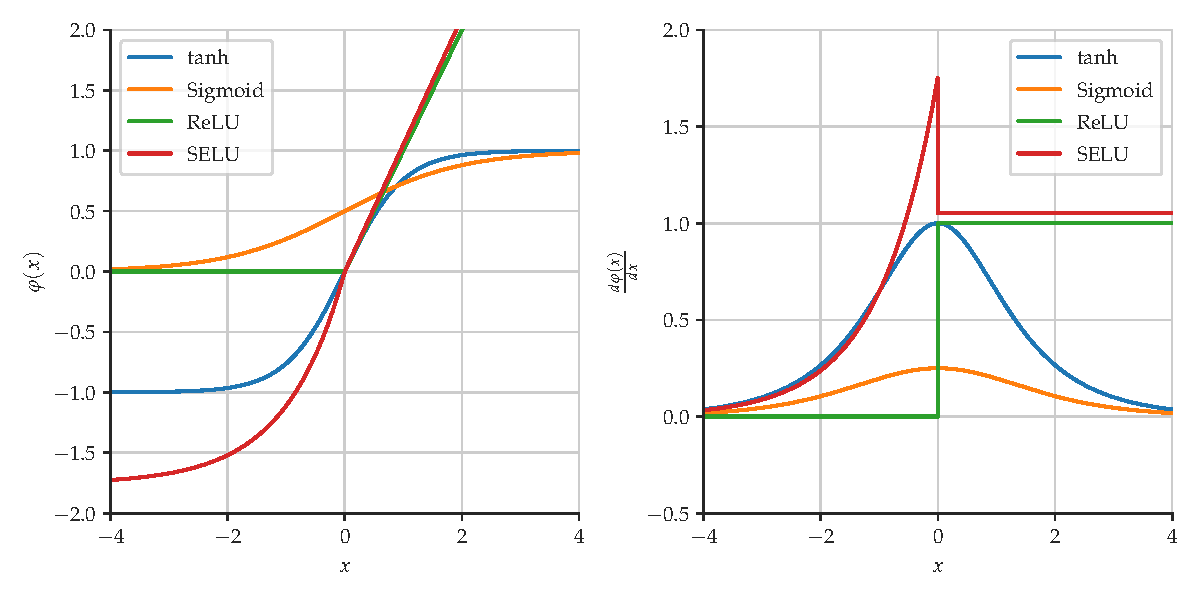
\includegraphics[scale = 0.7]{mlp-activations.pdf}
	\caption{À esquerda, algumas funções de ativação comuns em tarefas de predição e regressão para o neurônio \textit{Perceptron} e, à direita, suas derivadas}
	\label{fig:mlp-activations}
\end{figure}

É interessante mencionar o fato de que, assim como podemos selecionar uma gama de funções não-lineares para a ativação do neurônio, de forma a realizar transformações não-lineares na entrada, também é possível utilizar funções de ativação lineares, ou seja, realizar transformações lineares assim como os modelos clássicos de predição (como o AR e o ARMA) fazem. Nesse caso, a falta da não-linearidade tornaria muito difícil ou até mesmo impossibilitaria que sistemas mais complexos fossem descritos de forma aceitável por redes neurais artificiais desse tipo \cite{hornik1989multilayer}.

Tipicamente, uma rede neural MLP é composta por um número arbitrário $N_L$ de  camadas com $n$ neurônios do tipo \textit{Perceptron}, com a característica de que as saídas dos neurônios da $l$-ésima camada são propagadas para a frente, servindo como as entradas de todos os neurônios da camada seguinte ($l+1$). Esse processo é conhecido como \textit{feedforward}. Por isso, este tipo de rede é conhecida como totalmente conectada (ou densa). A figura \ref{fig:mlp-architecture} apresenta a estrutura típica das redes MLP.

\begin{figure}[!ht]
\centering
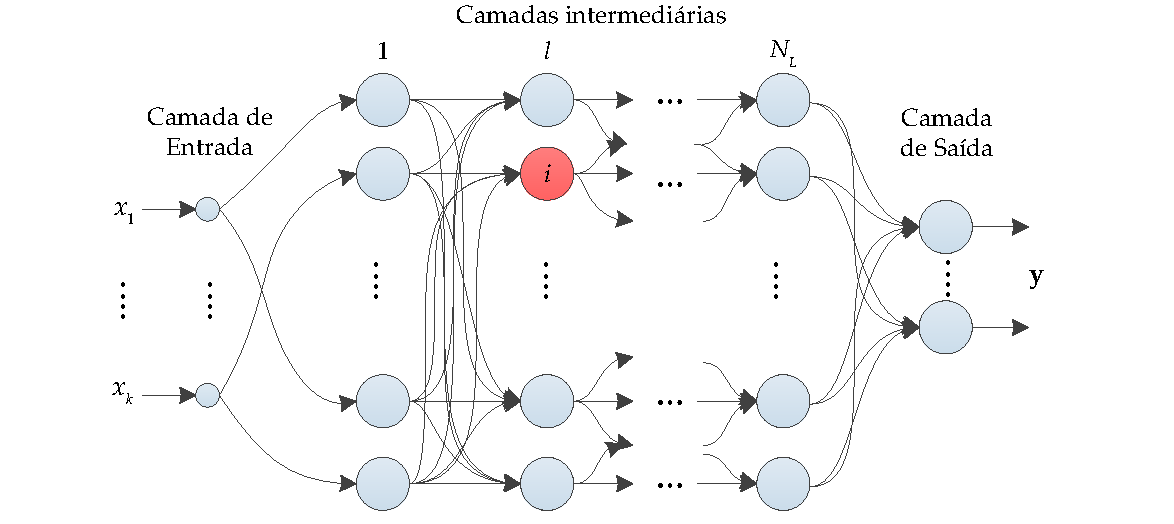
\includegraphics[scale = 0.8]{mlp-network.pdf}
\caption{Estrutura típica de uma rede MLP (figura extraída de \cite{boccato2013novas}) }
\label{fig:mlp-architecture}
\end{figure}

Pela figura vemos que, além das $N_L$ camadas intermediárias com neurônios \textit{Perceptron}, a estrutura das redes MLP contém uma camada de entrada, que possui ativação linear e apenas passa o atributo de entrada relacionado ao neurônio em específico ($x_1$, $x_2$, ..., $x_k$) para a primeira camada intermediária, e uma camada de saída que gera as respostas da rede neural para um vetor de entrada. A função de ativação da camada de saída e o número de neurônios presente nela dependem da tarefa a ser realizada pela MLP. Por exemplo, em aplicações de regressão é comum o uso de um ou mais neurônios (dependendo se a saída do preditor será um vetor com um ou mais instantes de tempo) com função de ativação linear. Já em aplicações de classificação, a função de ativação pode variar entre a função logística (utilizada no caso binário em que queremos saber se uma entrada pertence ou não a uma classe) e entre a função \textit{softmax} (que gera uma saída para cada classe, indicando a probabilidade de uma entrada pertencer à classe em específico) e, novamente, o número de neurônios de saída também varia com o tipo da classificação.

De forma similar a feita em (\ref{eq:mlp-out}), é possível representar a saída do $i$-ésimo neurônio da $l$-ésima camada intermediária, sendo que a anterior a esta possui $n_{l-1}$ neurônios, a $l$-ésima possui $n_l$ neurônios e a estrutura possui $N_L$ camadas intermediárias, da seguinte forma:
\begin{equation}
	y_{i}^{l} = \varphi^{l} \Big(\sum_{j=1}^{n_{l-1}} w_{ij}^{l} y_{j}^{l-1} + w_{i0}^{l} \Big)
\end{equation}
onde $w_{ij}^{l}$ representa o peso sináptico da conexão que liga o $j$-ésimo neurônio da camada $l-1$ ao $i$-ésimo neurônio da camada $l$, sendo que na primeira camada intermediária os sinais de entrada são os atributos do vetor de entrada, ou seja, $y_{j}^{0} = x_{j}$ com $j = 1, ..., k$ \cite{boccato2013novas}.

O processo de treinamento de uma rede neural artificial normalmente é realizado com sequências de vetores de entrada $\mathbf{x}$, chamadas de \textit{mini-batch}, e chamamos um período de treinamento de época (do inglês \textit{epoch}) \cite{geron2019hands}. No treinamento, os pesos sinápticos $\mathbf{w}$ são ajustados em um processo iterativo de forma a minimizar uma função custo $J(\mathbf{w})$ que representa uma medida do erro entre as saídas geradas pela rede e as saídas desejadas (vale mencionar que $\mathbf{w}$ é um vetor com todos os parâmetros da rede). No caso de um problema de regressão ou predição, é comum que a função custo a ser minimizada seja o Erro Quadrático Médio (MSE, do inglês \textit{Mean Squared Error}), assim, o problema envolve otimização não-linear irrestrita \cite{haykin2010neural}.

Para isso, é frequente o uso de algoritmos de otimização baseados em derivadas da função custo $J(\mathbf{w})$, como o método do gradiente descendente estocástico (SGD, do inglês \textit{stochastic gradient descent}), o método de Nesterov (NAG, do inglês \textit{Nesterov Accelerated Gradient}) e o algoritmo Adam (\textit{Adaptive Moment Estimation}) \cite{geron2019hands}. O famoso algoritmo de retropropagação (\textit{backpropagation}) do erro, cuja representação matemática também varia de acordo com o tipo de otimização, é empregado para viabilizar o cálculo das derivadas com relação aos pesos sinápticos dos neurônios situados nas camadas internas da rede, de forma que, para cada \textit{mini-batch} sejam atualizados todos os pesos de todos os neurônios da rede. 

Nesse caso, é comum dividirmos os métodos de otimização entre métodos de primeira ordem e de segunda ordem. Os métodos de primeira ordem utilizam as derivadas de primeira ordem da função custo, geralmente representadas com o uso do vetor gradiente:
\begin{equation}
	\nabla J(\mathbf{w}) = \Big[\frac{\partial J(\mathbf{w})}{\partial w_1} \; ...\;  \frac{\partial J(\mathbf{w})}{\partial w_n} \Big]^T
\end{equation}
assim, ao caminharmos na direção contrária à apontada pelo vetor $\nabla J(\mathbf{w})$ obtemos, de forma iterativa, a minimização desejada. Logo, a regra de atualização dos pesos pode ser dada pela forma básica:
\begin{equation}\label{mlp-w-basic}
	\mathbf{w}[k+1] \leftarrow \mathbf{w}[k] - \eta \nabla J \big[\mathbf{w}[k]\big]
\end{equation} 

Os algoritmos de otimização mencionados (SGD, Adam, NAG) utilizam variações da regra de atualização de $\mathbf{w}$ indicada em (\ref{mlp-w-basic}).

Para esta pesquisa, optamos por utilizar o algoritmo Nadam (\textit{Nesterov Adaptive Moment Estimation}) \cite{dozat2016incorporating}. O Nadam, como o nome já sugere, incorpora elementos dos algoritmos NAG e Adam, de forma a ter um passo de atualização adaptativo e com acúmulo dos gradientes mais recentes (semelhante a ideia de momento linear de uma partícula), com a utilização do "truque de Nesterov", desenvolvido pelo matemático russo Yurii Nesterov \cite{nesterov1983method}, onde o gradiente não é calculado sobre o ponto atual indicado pelo vetor $\mathbf{w}$, mas sim sobre um ponto levemente à frente, na mesma direção do momento. O conjunto de equações que descreve o algoritmo Nadam é dado por:
\begin{subequations}
\begin{equation}\label{eq:nadam-1}
 \mathbf{w}' = \mathbf{w} + \beta_{3} \mathbf{m}
\end{equation}
\begin{equation}\label{eq:nadam-2}
 \mathbf{m} \leftarrow \beta_{1}\mathbf{m} - (1 - \beta_{1}) \nabla_{\mathbf{w}}E(\mathbf{w}')
\end{equation}
\begin{equation}\label{eq:nadam-3}
 \mathbf{s} \leftarrow \beta_{2}\mathbf{s} - (1 - \beta_{2}) \nabla_{\mathbf{w}}E(\mathbf{w}') \otimes \nabla_{\mathbf{w}}E(\mathbf{w}') 
\end{equation}
\begin{equation}\label{eq:nadam-4}
\hat{\mathbf{m}} \leftarrow \frac{\mathbf{m}}{1 - \beta_{1}}
\end{equation}
\begin{equation}\label{eq:nadam-5}
\hat{\mathbf{s}} \leftarrow \frac{\mathbf{s}}{1 - \beta_{2}}
\end{equation}
\begin{equation}\label{eq:nadam-6}
 \mathbf{w} \leftarrow \mathbf{w} + \eta \hat{\mathbf{m}} \oslash \sqrt{\hat{\mathbf{s}} + \epsilon}
\end{equation}
\end{subequations}

A incorporação dos gradiantes passados no cálculo do próximo vetor $\mathbf{w}$ é através da equação (\ref{eq:nadam-2}), que define o vetor de momento $\mathbf{m}$. Assim, utilizando a analogia com o momento linear de uma partícula, o gradiente passa ter a ideia de uma força de aceleração que aumenta o valor do momento do vetor $\mathbf{w}$ caso este esteja indo para um ponto ótimo de mínimo local, escapando mais rapidamenete de regiões onde não há minimização significativa da função custo.

O hiperparâmetro $\beta_1$ presente em (\ref{eq:nadam-2}) serve tanto para evitar que $\mathbf{m}$ aumente de forma descontrolada, como também para fazer com que, através do termo $(1 - \beta_1)$, uma média exponencialmente decrescente de valores anteriores. Normalmente, $\beta_1$ é inicializado em $0.9$.

Já o vetor $\mathbf{s}$, definido em (\ref{eq:nadam-3}), serve para evitar que o algoritmo de otimização caminhe com uma direção que não aponte para o ponto ótimo mencionado anteriormente. Além disso, para evitar que esse ajuste na direção cause uma perda significativa na rapidez de convergência do algoritmo, utiliza-se os termos $\beta_2$ e $(1 - \beta_2)$, ou seja, um decaimento exponencial nos valores passados de $\mathbf{s}$. Nesse caso, o hiperparâmetro $\beta_2$ é inicializado em $0.999$ e $\epsilon$ em $10^{-7}$ (para evitar uma divisão por zero).

Por fim, as equações (\ref{eq:nadam-4}) e (\ref{eq:nadam-5}) servem para inicializar os vetores $\mathbf{m}$ e $\mathbf{s}$ com valores próximos de $1$, impulsionando a atualização deles no começo do treinamento.

É importante mencionar que os métodos de otimização aqui mencionados são métodos de busca local, ou seja, têm convergência esperada para um mínimo local, que não necessariamente é o mínimo global da função custo para a aplicação. Dizemos também que esses pontos mínimos possuem "bacias de atração" que, para valores adequados da taxa de aprendizado $\eta$, atrai o vetor de parâmetros $\mathbf{w}$ \cite{hastie2009elements}.

Algo presente durante o treinamento da rede neural é, ou desaparecimento dos gradientes (do inglês \textit{vanishing gradients problem}) nas camadas inferiores da rede, ou o aumento desenfreado desses gradientes (do inglês \textit{exploding gradients problem}) nas camadas citadas, que é mais comum para redes recorrentes. Para evitar que isso ocorra, normalmente são utilizadas camadas que realizam uma normalização do \textit{batch} de vetores de entrada (BN, do inglês \textit{Batch Normalization}), sendo posicionadas antes ou depois das camadas intermediárias da rede \cite{geron2019hands}.

O que a normalização faz, é centrar todas as instâncias de vetores de entrada presentes no atual \textit{mini-batch} ao redor do zero e as normaliza. Logo, podemos representar a transformação aplicada com as seguintes equações:
\begin{subequations}
\begin{equation}\label{eq:bn-1}
 \boldsymbol{\mu}_{B} = \frac{1}{d} \sum_{i=1}^{d} \mathbf{x}_{i} 
\end{equation}
\begin{equation}\label{eq:bn-2}
\boldsymbol{\sigma}_{B}^{2} = \frac{1}{d} \sum_{i=1}^{d} (\mathbf{x}_{i} - \boldsymbol{\mu}_{B})^2 
\end{equation}
\begin{equation}\label{eq:bn-3}
\hat{\mathbf{x}}_{i} = \frac{\mathbf{x}_{i} - \boldsymbol{\mu}_{B}}{\sqrt{\boldsymbol{\sigma}_{B} + \epsilon}}
\end{equation}
\begin{equation}\label{eq:bn-4}
\mathbf{z}_{i} = \boldsymbol{\gamma} \otimes \hat{\mathbf{x}}_{i} + \boldsymbol{\beta}
\end{equation}
\end{subequations}
sendo $\boldsymbol{\mu}_{B}$ e $\boldsymbol{\sigma}_{B}$ os vetores com as médias e desvio-padrão para cada atributo de entrada do atual \textit{mini-batch} (este contendo $d$ vetores $\mathbf{x}$), $\hat{\mathbf{x}}_{i}$ é o $i$-ésimo vetor de entrada centrado em zero e normalizado, $\boldsymbol{\gamma}$ é o vetor que pondera cada um dos atributos de $\hat{\mathbf{x}}_{i}$, $\boldsymbol{\beta}$ tem um termo de \textit{offset} para cada atributo normalizado, $\epsilon$ novamente é um termo pequeno (geralmente na ordem de $10^{-5}$) para evitar uma divisão por zero e, por fim, $\mathbf{z}_{i}$ é a saída da camada de \textit{batch normalization}.

Os hiperparâmetros $\boldsymbol{\beta}$ e $\boldsymbol{\gamma}$ controlam o deslocamento e o escalonamento, respectivamente, de cada atributo para um vetor de entrada. Essas variáveis são parametrizadas durante o treinamento da rede neural de forma bem eficiente dependendo da quantidade e do tamanho dos \textit{mini-batches}. 

Também vale mencionar que, para o conjunto de dados de validação, ou seja, o conjunto de dados que, após o ajuste dos pesos $\mathbf{w}$ no conjunto de treinamento, é verificado se a rede neural está generalizando os resultados, evitando o sobreajuste (do inglês \textit{overfitting}), são calculados outros vetores de valores de média ($\boldsymbol{\mu}_{B}'$) e desvio-padrão ($\boldsymbol{\sigma}_{B}'$). Assim, o processo descrito anteriormente também é realizado sobre esses dados.

Por fim, o grande apelo das redes \textit{Multilayer Perceptron} é que elas tem a capacidade de aproximação universal, ou seja, são capazes de aproximar qualquer mapeamento contí\-nuo num domínio compacto com um nível de erro arbitrariamente pequeno. Até mesmo uma MLP com uma única camada intermediária e camada de saída linear já possui esta capacidade \cite{cybenko1989approximation, hornik1989multilayer}. Infelizmente, esse teorema não indica a quantidade de neurônios necessária na(s) camada(s) intermediária(s), muito menos um método para ajustar o vetor $\mathbf{w}$ da rede para garantir a solução ótima.

Além disso, para o propósito deste trabalho de pesquisa, que envolve sistemas dinâmicos, ter acesso a um histórico e a uma memorização dos padrões anteriores de entrada, na teoria, aumentaria a precisão da predição das séries temporais. Mesmo que as redes MLP tenham capacidade de aproximação universal, é possível aumentar a eficiência desse processo caso fossem utilizadas estruturas recorrentes \cite{connor1994recurrent}.

Logo, incluímos na análise alguns modelos de redes neurais recorrentes. Discutiremos mais sobre a estrutura e o funcionamento delas na próxima seção.

\subsubsection{Redes Recorrentes \textit{Long Short-term Memory} (LSTM)}
Diferentemente das redes MLP que são \textit{feedforward}, ou seja, que não reutilizam a informação processada dos padrões anteriores para gerar a próxima saída, a ideia central das redes recorrentes é que elas têm estruturas computacionais que podem armazenar os estados anteriores dos neurônios, possuindo também portas não-lineares que regulam o fluxo de informação de entrada e de saída da célula computacional \cite{haykin2010neural}. Uma representação possível de uma célula de uma rede recorrente pode ser vista na Figura \ref{fig:recorrente}. Note que a saída é realimentada (com um atraso temporal) para a entrada do próprio neurônio.


Em especial, as redes LSTM se mostram atraentes pela possibilidade de criar e explorar memórias de curto e de longo prazo. A estrutura da célula ou camada LSTM, assim como as equações presentes nela, são apresentadas na Figura \ref{fig:lstm}. 
\noindent{
\begin{figure}[H]
\begin{minipage}{0.5\textwidth}
\begin{center}   
\begin{tikzpicture}[x=0.65pt,y=0.65pt,yscale=-1,xscale=1]
%uncomment if require: \path (0,300); %set diagram left start at 0, and has height of 300

%Straight Lines [id:da1554249944842837] 
\draw    (320.58,202.18) -- (320.19,163.18) ;
\draw [shift={(320.17,161.18)}, rotate = 449.42] [color={rgb, 255:red, 0; green, 0; blue, 0 }  ][line width=0.75]    (10.93,-3.29) .. controls (6.95,-1.4) and (3.31,-0.3) .. (0,0) .. controls (3.31,0.3) and (6.95,1.4) .. (10.93,3.29)   ;
%Shape: Circle [id:dp7598463649301769] 
\draw   (295.17,136.18) .. controls (295.17,122.38) and (306.36,111.18) .. (320.17,111.18) .. controls (333.97,111.18) and (345.17,122.38) .. (345.17,136.18) .. controls (345.17,149.99) and (333.97,161.18) .. (320.17,161.18) .. controls (306.36,161.18) and (295.17,149.99) .. (295.17,136.18) -- cycle ;
%Straight Lines [id:da5775924503019426] 
\draw    (320.17,111.18) -- (319.61,73.18) ;
\draw [shift={(319.58,71.18)}, rotate = 449.16] [color={rgb, 255:red, 0; green, 0; blue, 0 }  ][line width=0.75]    (10.93,-3.29) .. controls (6.95,-1.4) and (3.31,-0.3) .. (0,0) .. controls (3.31,0.3) and (6.95,1.4) .. (10.93,3.29)   ;
%Curve Lines [id:da6508772564279707] 
\draw    (340.58,116.18) .. controls (404.93,98.36) and (405.58,137.39) .. (343.48,152.73) ;
\draw [shift={(341.58,153.18)}, rotate = 346.81] [color={rgb, 255:red, 0; green, 0; blue, 0 }  ][line width=0.75]    (10.93,-3.29) .. controls (6.95,-1.4) and (3.31,-0.3) .. (0,0) .. controls (3.31,0.3) and (6.95,1.4) .. (10.93,3.29)   ;
%Straight Lines [id:da12570537723123754] 
\draw    (295.17,136.18) -- (345.17,136.18) ;
%Straight Lines [id:da42455472986521403] 
\draw    (304.58,129.68) -- (320.58,129.68) ;
%Straight Lines [id:da862734419251405] 
\draw    (320.58,129.68) -- (330.58,119.68) ;

% Text Node
\draw (392,116) node [anchor=north west][inner sep=0.75pt]   [align=left] {$y(t-1)$};
% Text Node
\draw (309,51) node [anchor=north west][inner sep=0.75pt]   [align=left] {$y(t)$};
% Text Node
\draw (309,206) node [anchor=north west][inner sep=0.75pt]   [align=left] {$x(t)$};
% Text Node
\draw (309,137.5) node [anchor=north west][inner sep=0.75pt]   [align=left] {$\sum$};
\end{tikzpicture}
\caption{Célula da rede recorrente}
\label{fig:recorrente}
\end{center}
\end{minipage}
\begin{minipage}{0.5\textwidth}
\begin{center}
\begin{tikzpicture}[
    % GLOBAL CFG
    font=\sf \scriptsize,
    >=LaTeX,
    % Styles
    cell/.style={% For the main box
        rectangle, 
        rounded corners=5mm, 
        draw,
        very thick,
        },
    operator/.style={%For operators like +  and  x
        circle,
        draw,
        inner sep=-0.5pt,
        minimum height =.2cm,
        },
    function/.style={%For functions
        ellipse,
        draw,
        inner sep=1pt
        },
    ct/.style={% For external inputs and outputs
        circle,
        draw,
        line width = .75pt,
        minimum width=1cm,
        inner sep=1pt,
        },
    gt/.style={% For internal inputs
        rectangle,
        draw,
        minimum width=4mm,
        minimum height=3mm,
        inner sep=1pt
        },
    mylabel/.style={% something new that I have learned
        font=\scriptsize\sffamily
        },
    ArrowC1/.style={% Arrows with rounded corners
        rounded corners=.25cm,
        thick,
        },
    ArrowC2/.style={% Arrows with big rounded corners
        rounded corners=.5cm,
        thick,
        },
    scale = 0.95
    ]

%Start drawing the thing...    
    % Draw the cell: 
    \node [cell, minimum height =4cm, minimum width=6cm] at (0,0){} ;

    % Draw inputs named ibox#
    \node [gt] (ibox1) at (-2,-0.75) {$\sigma$};
    \node [gt] (ibox2) at (-1.5,-0.75) {$\sigma$};
    \node [gt, minimum width=1cm] (ibox3) at (-0.5,-0.75) {$\tanh$};
    \node [gt] (ibox4) at (0.5,-0.75) {$\sigma$};

   % Draw opérators   named mux# , add# and func#
    \node [operator] (mux1) at (-2,1.5) {$\times$};
    \node [operator] (add1) at (-0.5,1.5) {+};
    \node [operator] (mux2) at (-0.5,0) {$\times$};
    \node [operator] (mux3) at (1.5,0) {$\times$};
    \node [function] (func1) at (1.5,0.75) {$\tanh$};

    % Draw External inputs? named as basis c,h,x
    \node[] (c) at (-4,1.5) {$\mathbf{c}(t-1)$};
    \node[] (h) at (-4,-1.5) {$\mathbf{h}(t-1)$};
    \node[] (x) at (-2.5,-3) {$\mathbf{x}(t)$};

    % Draw External outputs? named as basis c2,h2,x2
    \node[] (c2) at (4,1.5) {$\mathbf{c}(t)$};
    \node[] (h2) at (4,-1.5) {$\mathbf{h}(t)$};
    \node[] (x2) at (2.5,3) {$\mathbf{h}(t)$};
    
    % Draw internals functions, named as basis fi,ii,ci,oi
    \node[] (fi) at (-2.35,-0.25) {$\mathbf{f}(t)$};
    \node[] (ii) at (-1.5,0.2) {$\mathbf{i}(t)$};
    \node[] (ci) at (-0.1,-0.35) {$\mathbf{\tilde{c}}(t)$};
	\node[] (oi) at (0.5,0.2) {$\mathbf{o}(t)$};      
	
    % Draw equations named as basis fe,ie,cie,ce,oe,he
    \node[] (fe) at (0.5,-2.5) {$\mathbf{f}(t) = \sigma(\mathbf{W}_f [\mathbf{h}(t-1), \mathbf{x}(t)] + \mathbf{b}_f)$};
    \node[] (ie) at (0.5,-3) {$\mathbf{i}(t) = \sigma(\mathbf{W}_i [\mathbf{h}(t-1), \mathbf{x}(t)] + \mathbf{b}_i)$};
    \node[] (cie) at (0.5,-3.5) {$\mathbf{\tilde{c}}(t) = \sigma(\mathbf{W}_c [\mathbf{h}(t-1), \mathbf{x}(t)] + \mathbf{b}_c)$};	      
    \node[] (ce) at (0.5,-4) {$\mathbf{c}(t) = \mathbf{f}(t) \otimes \mathbf{c}(t-1) + \mathbf{i}(t) \otimes \mathbf{\tilde{c}}(t)$};
    \node[] (oe) at (0.5,-4.5) {$\mathbf{o}(t) = \sigma(\mathbf{W}_o [\mathbf{h}(t-1), \mathbf{x}(t)] + \mathbf{b}_o)$};
    \node[] (he) at (0.5,-5) {$\mathbf{h}(t) = \mathbf{o}(t) \otimes \tanh (\mathbf{c}(t))$};	 
    
% Start connecting all.
    %Intersections and displacements are used. 
    % Drawing arrows    
    \draw [ArrowC1] (c) -- (mux1) -- (add1) -- (c2);

    % Inputs
    \draw [ArrowC2] (h) -| (ibox4);
    \draw [ArrowC1] (h -| ibox1)++(-0.5,0) -| (ibox1); 
    \draw [ArrowC1] (h -| ibox2)++(-0.5,0) -| (ibox2);
    \draw [ArrowC1] (h -| ibox3)++(-0.5,0) -| (ibox3);
    \draw [ArrowC1] (x) -- (x |- h)-| (ibox3);

    % Internal
    \draw [->, ArrowC2] (ibox1) -- (mux1);
    \draw [->, ArrowC2] (ibox2) |- (mux2);
    \draw [->, ArrowC2] (ibox3) -- (mux2);
    \draw [->, ArrowC2] (ibox4) |- (mux3);
    \draw [->, ArrowC2] (mux2) -- (add1);
    \draw [->, ArrowC1] (add1 -| func1)++(-0.5,0) -| (func1);
    \draw [->, ArrowC2] (func1) -- (mux3);

    %Outputs
    \draw [->, ArrowC2] (mux3) |- (h2);
    \draw [->] (add1) |- (c2);
    \draw (c2 -| x2) ++(0,-0.1) coordinate (i1);
    \draw [-, ArrowC2] (h2 -| x2)++(-0.5,0) -| (i1);
    \draw [->, ArrowC2] (i1)++(0,0.2) -- (x2);

\end{tikzpicture}
\caption{Estrutura e equações de uma célula/camada LSTM}
\label{fig:lstm}
\end{center}
\end{minipage}
\end{figure}
}
As LSTMs manipulam o vetor $\mathbf{c}(t)$, aprendendo durante o treinamento o que deve ser guardado nele, o que deve ser descartado e o que deve ser aproveitado para gerar a saída $\mathbf{h}(t)$. Dessa forma, podemos dizer que a atualização do vetor de estados $\mathbf{c}(t)$ é feita com o descarte de informações e a incorporação de novidades vindas da entrada. 

À semelhança das redes MLP, o treinamento de uma LSTM também é realizado através de algoritmos de otimização baseados em derivadas da função custo; a diferença é que agora é necessário propagar as derivadas ao longo da estrutura e, também, ao longo do tempo devido às realimentações. O algoritmo BPTT (\textit{backpropagation-through-time}) representa a extensão do backpropagation para o cenário das redes recorrentes \cite{geron2019hands}. 

\section{Sistemas com Dinâmica Caótica}
Como dito anteriormente, sistemas com dinâmica cáotica se destacam pois, apesar de serem determinísticos, apresentam dependência sensitiva em relação às condições iniciais (DSCI). Dessa forma, duas trajetórias que partem de posições relativamente próximas no espaço de estados podem evoluir de uma forma totalmente distinta devido às não-linearidades presentes que amplificam as diferenças entre essas condições iniciais \cite{fiedler1994caos}.

De forma resumida, a dinâmica caótica é marcada pela presença dos seguintes aspectos \cite{attux2001dinamica}:
\begin{enumerate}
\item Forte sensibilidade com respeito às condições iniciais;
\item A evolução temporal das variáveis de estado (parâmetros de ordem do sistema) é rápida e tem uma aparência errática;
\item Um sinal originado por um sistema caótico tem espectro de potências contínuo e de faixa larga;
\item Há uma produção de informação por parte do sistema;
\item Dão origem a atratores estranhos (estruturas topológicas que ditam a evolução temporal do fluxo de um sistema caótico) \cite{ruelle1971nature}.
\end{enumerate}

\section{Próximos Passos}

Como nessa primeira parte da iniciação o foco foi uma pesquisa bibliográfica dos temas a serem estudados nela, a segunda metade será voltada para a aplicação em si da predição das séries temporais de sistemas caóticos.

Para os experimentos computacionais, optamos pelas séries temporais do Mapa Logístico, descrito pelo cientista Robert May \cite{may1976simple}, o Mapa de Hénon, apresentado pelo astronômo e matemático francês Michel Hénon \cite{henon1976two}, a famosa série Mackey-Glass, dos cientistas Michael Mackey e Leon Glass \cite{mackey1977oscillation}, e o clássico Sistema de Lorenz, um dos  mais incríveis e fundamentais trabalhos de sistemas caóticos, introduzido pelo matemático e meteorologista Edward Norton Lorenz \cite{lorenz1963deterministic}, de forma a criar cenários diversificados para a análise do comportamento das redes neurais, com sistemas a tempo contínuo (Sistema de Lorenz e Equações de Mackey-Glass) e sistemas a tempo discreto (Mapa de Hénon e Mapa Logístico).

Em seguida, determinaremos aspectos mais fundamentais das redes neurais que serão utilizadas, como, por exemplo, a arquitetura empregada, assim como as métricas para o treinamento e análise. Para essa etapa, também planejamos um estudo das redes GRU (do inglês \textit{Gated Recurrent Unit}) \cite{cho2014learning} e ESN (do inglês \textit{Echo State Network}) \cite{jaeger2007echo}, sendo que esta última, em outros trabalhos de pesquisa, já indicou um bom desempenho preliminar no contexto de predição de séries temporais originadas por sistemas caóticos \cite{boccato2013novas}.

Após isso, faremos a aplicação das redes neurais à predição das séries escolhidas, avaliando a sensibilidade paramétrica de cada estrutura na busca das melhores configurações, a fim de traçar um quadro comparativo entre as técnicas consideradas. 

Por fim, compilaremos os resultados no relatório final, de forma a conter uma discussão ampla e representativa dos ensaios realizados e das conclusões obtidas. 

\bibliographystyle{ieeetr}

\bibliography{bib}

\end{document}